\subsection{Local Properties}
\label{sec:localProperties}

\floatstyle{boxed}
\restylefloat{figure}

\begin{figure}\small
\begin{inv}
A response \Resp{p}{c}{a}{x}, where $p = c.parent$, can be sent from $p$ only
if
\begin{enumerate}
\item a request \Req{c}{p}{a}{z} was received from $c$,
\item $p$ is not waiting for any response for address $a$ from $c$, and
\item $x > y$, where $p.dir[c][a] = y$ just before sending the response
\end{enumerate}
\label{pSendRespPre}
\end{inv}
\begin{inv}
A response \Resp{c}{p}{a}{x}, where $p = c.parent$, can be sent from $c$ only
if $x < y$, where $c.state[a] = y$ just before sending the
response\label{cSendRespPre1}
\end{inv}
\begin{inv}
If $c$ has sent a request \Req{c}{p}{a}{x}, then $c$ can send a response
\Resp{c}{p}{a}{y} only on receiving a request from $p$ for address $a$.
\label{cSendRespPre2}
\end{inv}
%\caption{Local-Properties for sending responses}
%\label{sendResp}
%\end{figure}
%
%\begin{figure}\small
\begin{inv}
If a response \Resp{p}{c}{a}{x} is sent from $p$, then $p.dir[c][a] \gets x$\label{cSendRespPost}
\end{inv}
\begin{inv}
If \Resp{c}{p}{a}{x} is sent $c.state[a] \gets x$\label{pSendRespPost}
\end{inv}
\begin{inv}
On receiving a response \Resp{c}{p}{a}{x}, where $p = c.parent$, $p.dir[c][a]
\gets x$\label{pRecvResp}
\end{inv}
\begin{inv}
On receiving a response \Resp{p}{c}{a}{x}, where $p = c.parent$, $c.state[c]
\gets x$\label{cRecvResp}
\end{inv}
\begin{inv}
$c.state[a]$ can change only on $c$ sending a response to or receiving a
response from $c.parent$\label{cState}
\end{inv}
\begin{inv}
$p.dir[c][a]$ can change only on $p$ sending or receiving a response from
its child $c$\label{pState}
\end{inv}
%\caption{Local-Properties for state changes}
%\label{stateChange}
%\end{figure}
%
%\begin{figure}\small
\begin{inv}
\Req{p}{c}{a}{x}, where $p = c.parent$, can be sent only if $x < p.dir[c][a]$\label{pSendReqPre}
\end{inv}
\begin{inv}
If \Req{p}{c}{a}{x}, where $p = c.parent$, is received, if $x \ge c.state[a]$,
then the request is dropped\label{pSendReqPost}
\end{inv}
\begin{inv}
\Req{c}{p}{a}{x}, where $p = c.parent$, can be sent only if $x > c.state[a]$\label{cSendReqPre}
\end{inv}
\begin{inv}
If \Req{c}{p}{a}{x}, where $p = c.parent$, is received, it $x \le p.state[a]$,
then the request is dropped\label{cSendReqPost}
\end{inv}
\begin{inv}
A request can be sent by a cache node $n$ for address $n$ to another cache node $m$ only if
no $n$ is not waiting for a response for address $a$ from $m$.
\label{nodoublereq}
\end{inv}
\caption{Local-Properties useful in proving the correctness of MSI protocol}
\label{sendReq}
\end{figure}

The Local-Properties capture the core properties of the distributed MSI
protocol given in Section \ref{sec:DistributedMsi}, and the requirements
mentioned in Section \ref{sec:network}. We will use the violation of
Local-Properties \ref{pSendRespPre} and \ref{cSendRespPre2} as examples to
illustrate the importance of local properties.  In our usual system, let's say
$c_1.state[a] = p.dir[c_1][a] = S$, $c_2.state[a] = p.dir[c_2][a] = I$.

\floatstyle{plain}
\restylefloat{figure}
\begin{figure}
\centering
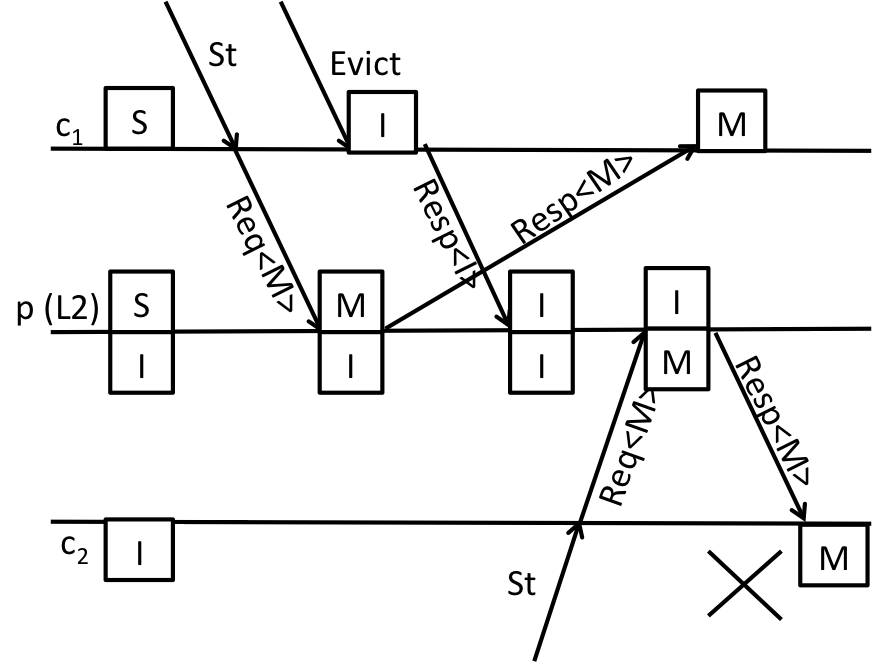
\includegraphics[scale=0.34]{checkit}
\caption{Effect of violating Invariant \ref{cSendRespPre2} (child evicts a ``pending'' line)}
\label{checkit}
\end{figure}
\floatstyle{boxed}
\restylefloat{figure}

Let $c_1$ receive a store request for address $a$. It sends an upgrade-to-$M$
request to $p$. Then $c_1$ violates \ref{cSendRespPre2} and evicts $a$ to
replace it with another address. It sends a downgrade to $I$ response for
address $a$ to $p$.  Meanwhile $p$ has sent an upgrade-to-$M$ response to
$c_1$. $c_1$ receives the response and upgrades address $a$ to $M$. $p$ then
receives the downgrade to $I$ response form $c_1$. So $p$ now assumes that
$c_1$ is in $I$ while in reality, $c_1$ is in $M$. This breaks Invariant
\ref{conservative} which creates the problems described earlier. This is shown
in Figure \ref{checkit}

\floatstyle{plain}
\restylefloat{figure}
\begin{figure}
\centering
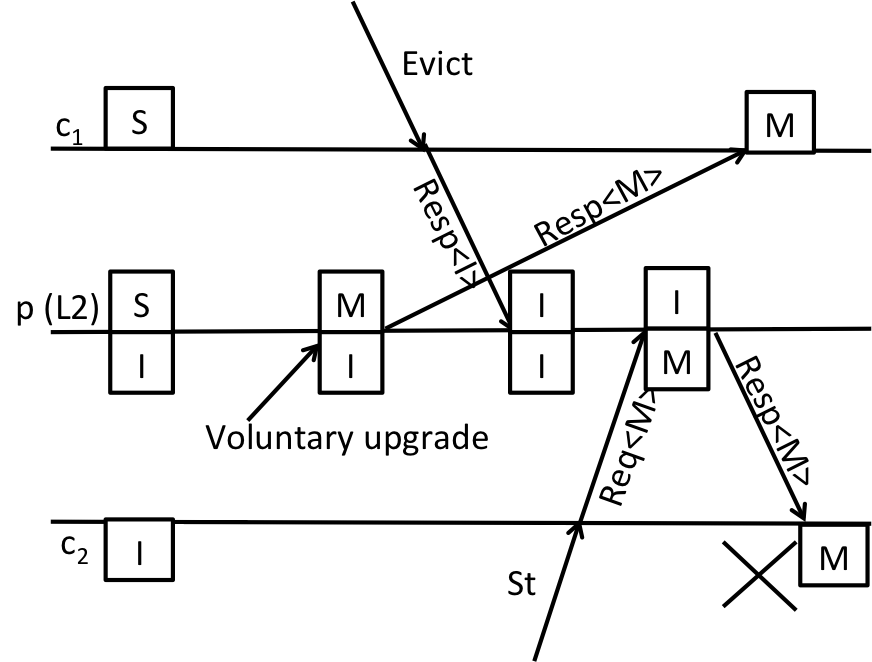
\includegraphics[scale=0.34]{checkit2}
\caption{Effect of violating Invariant \ref{pSendRespPre} (parent sends a voluntary response)}
\label{checkit2}
\end{figure}
\floatstyle{boxed}
\restylefloat{figure}

Let's say $p$ violates \ref{pSendRespPre} and voluntarily sends an
upgrade-to-$M$ response for address $a$ to $c_1$.  Meanwhile, $c_1$ evicts $a$
to replace it with another address. $c_1$ then gets the upgrade-to-$M$ response
from $p$ while $p$ gets the downgrade to $I$ response, breaking Invariant
\ref{conservative} again. This is shown in Figure \ref{checkit2}.

In general, any crossing of response messages between a cache and its parent,
like the ones shown in Figures \ref{checkit} and \ref{checkit2} results in
violation of Invariant \ref{conservative}.
